% On découpe ce document complexe en plusieurs sous-fichiers séparés.
% Cela permettra notamment de réarranger les transparents facilement
% lors de l'élaboration du document.

% La définition de la classe beamer avec tous les styles afférents
%%%%%%%%%%%%%%%%%%%%%%%%%%%%%%%%%%%%%%%%%
% Beamer Presentation
% LaTeX Template
% Version 1.0 (10/11/12)
%
% This template has been downloaded from:
% http://www.LaTeXTemplates.com
%
% License:
% CC BY-NC-SA 3.0 (http://creativecommons.org/licenses/by-nc-sa/3.0/)
%
%%%%%%%%%%%%%%%%%%%%%%%%%%%%%%%%%%%%%%%%%

%----------------------------------------------------------------------------------------
%	PACKAGES AND THEMES
%----------------------------------------------------------------------------------------

\RequirePackage{currfile} 


\documentclass{beamer}


\mode<presentation> {

% The Beamer class comes with a number of default slide themes
% which change the colors and layouts of slides. Below this is a list
% of all the themes, uncomment each in turn to see what they look like.

%\usetheme{default}
%\usetheme{AnnArbor}
%\usetheme{Antibes}
%\usetheme{Bergen}
%\usetheme{Berkeley}
%\usetheme{Berlin}
%\usetheme{Boadilla}
%\usetheme{CambridgeUS}
%\usetheme{Copenhagen}
%\usetheme{Darmstadt}
%\usetheme{Dresden}
%\usetheme{Frankfurt}
%\usetheme{Goettingen}
%\usetheme{Hannover}
%\usetheme{Ilmenau}
%\usetheme{JuanLesPins}
%\usetheme{Luebeck}
%\usetheme{Madrid}		
%\usetheme{Malmoe}
%\usetheme{Marburg}
%\usetheme{Montpellier}
%\usetheme{PaloAlto}
%\usetheme{Pittsburgh}
%\usetheme{Rochester}
%\usetheme{Singapore}
%\usetheme{Szeged}
\usetheme{Warsaw}

% As well as themes, the Beamer class has a number of color themes
% for any slide theme. Uncomment each of these in turn to see how it
% changes the colors of your current slide theme.

%\usecolortheme{albatross}
%\usecolortheme{beaver}
%\usecolortheme{beetle}
%\usecolortheme{crane}
%\usecolortheme{dolphin}
%\usecolortheme{dove}
%\usecolortheme{fly}
%\usecolortheme{lily}
%\usecolortheme{orchid}
%\usecolortheme{rose}
%\usecolortheme{seagull}
%\usecolortheme{seahorse}
\usecolortheme{whale}
%\usecolortheme{wolverine}

%\setbeamertemplate{footline} % To remove the footer line in all slides uncomment this line
%\setbeamertemplate{footline}[frame number] % To replace the footer line in all slides with a simple slide count uncomment this line

%\setbeamertemplate{navigation symbols}{} % To remove the navigation symbols from the bottom of all slides uncomment this line

\setbeamercovered{transparent} % Fait apparaître les animations en grisé (utile pour la conception, mais peut être commenté lors de la remise du document final)

% Pour utiliser une police à empattements partout
\usefonttheme{serif}

% Pour rajouter la numérotation des frames dans les pieds de page
\newcommand*\oldmacro{}%
\let\oldmacro\insertshorttitle%
\renewcommand*\insertshorttitle{%
  \oldmacro\hfill%
  \insertframenumber\,/\,\inserttotalframenumber}

}

\usepackage{graphicx} % Allows including images
\usepackage{booktabs} % Allows the use of \toprule, \midrule and \bottomrule in tables




% Les autres packages utiles  notamment pour le français, les accents ou Python
\usepackage{natbib}         % Pour la bibliographie
\usepackage{url}            % Pour citer les adresses web
\usepackage[T1]{fontenc}    % Encodage des accents
\usepackage[utf8]{inputenc} % Lui aussi
\usepackage[frenchb]{babel} % Pour la traduction française
\usepackage{numprint}       % Histoire que les chiffres soient bien

\usepackage{amsmath}        % La base pour les maths
\usepackage{mathrsfs}       % Quelques symboles supplémentaires
\usepackage{amssymb}        % encore des symboles.
\usepackage{amsfonts}       % Des fontes, eg pour \mathbb.

\usepackage{cancel}

%\usepackage[svgnames]{xcolor} % De la couleur

%%% Si jamais vous voulez changer de police: décommentez les trois 
%\usepackage{tgpagella}
%\usepackage{tgadventor}
%\usepackage{inconsolata}

%%% Pour L'utilisation de Python
\usepackage{minted}
\usemintedstyle{friendly}

\usepackage{graphicx} % inclusion des graphiques
\usepackage{wrapfig}  % Dessins dans le texte.

\usepackage{tikz}     % Un package pour les dessins (utilisé pour l'environnement {code})
\usepackage[framemethod=TikZ]{mdframed}

% Les macros et raccourcis personnels
% Ce fichier contient toutes les macros que vous pouvez avoir envie de définir
% si vous les utilisez plusieurs fois dans le document.

\PassOptionsToPackage{svgnames}{color}

% Un environnement pour bien présenter le code informatique
\newenvironment{code}{%
\begin{mdframed}[linecolor=green,innerrightmargin=30pt,innerleftmargin=30pt,
backgroundcolor=black!5,
skipabove=10pt,skipbelow=10pt,roundcorner=5pt,
splitbottomskip=6pt,splittopskip=12pt]
}{%
\end{mdframed}
}

% Un raccourci pour composer les unités correctement (en droit)
% Exemple: $v = 10\U{m.s^{-1}}$
\newcommand{\U}[1]{~\mathrm{#1}}

% Les guillemets \ofg{par exemple}
\newcommand{\ofg}[1]{\og{}#1\fg{}}

% Le d des dérivées doit être droit: \frac{\dd x}{\dd t}
\newcommand{\dd}{\text{d}}

% La dérivée temporelle, tellement courante en physique, avec les d droits
\newcommand{\ddt}[1]{\frac{\dd #1}{\dd t}}

% Des parenthèses, crochets et accolades qui s'adaptent automatiquement à la
% taille de ce qu'il y a dedans
\newcommand{\pa}[1]{\left(#1\right)}
\newcommand{\pac}[1]{\left[#1\right]}
\newcommand{\paa}[1]{\left\{#1\right\}}

% Un raccourci pour écrire une constante
\newcommand{\cte}{\text{C}^{\text{te}}}

% Pour faire des indices en mode texte (comme les énergie potentielles)
\newcommand{\e}[1]{_{\text{#1}}}

% Le produit vectoriel a un nom bizarre:
\newcommand{\vectoriel}{\wedge}

\AtBeginSection[]{
  \begin{frame}
  \vfill
  \centering
  \begin{beamercolorbox}[sep=8pt,center,shadow=true,rounded=true]{title}
    \usebeamerfont{title}\insertsectionhead\par%
  \end{beamercolorbox}
  \vfill
  \end{frame}
}


% On définit le titre et l'auteur du document

% L'argument optionnel (entre crochets) donne le titre qui sera mis sur chaque slide
\title[GitHub en CPGE]{GitHub et GitHub classroom \\
pour la gestion des TP en CPGE}
\author{Jean-Julien \textsc{Fleck}} % Votre nom
\institute{Lycée Kléber}
\date{Luminy 2019}

% On démarre le document proprement dit
\begin{document}

% La page de titre et la table des matières
% Rien d'autre à faire qu'afficher le titre
\begin{frame}
\titlepage 
\end{frame}


% La table des matières utilise ce que vous donnez aux commandes \section et 
% \subsection tout au long de la présentation.
\begin{frame}
\frametitle{Plan de l'exposé} 
\tableofcontents 
\end{frame}


% L'intro: comment on procédait jusque là
% Titre de la premiere partie
\section{Gestion des TP, ancien protocole}

%%%%%%%%%%%%%%%%%%%%%%%%%%%%%%%%%%%%%%%%%%%%%%%%
% Diapo Git
%%%%%%%%%%%%%%%%%%%%%%%%%%%%%%%%%%%%%%%%%%%%%%%%
\begin{frame}
	\frametitle{Gestion des TP}
	\framesubtitle{Organisation avant GitHub}

	\begin{itemize}[<+->]
		\item	 Dossier de chaque TP distribué (depuis un ordi du lycée) sur les sessions des élèves (sur les ordis du lycée)

		\item  Travail des élèves sur les ordis du lycée et récupération sur clé USB pour bosser à la maison

		\item Ramassage des dossiers des élèves (depuis un ordi du lycée)

	\end{itemize}

\end{frame}


%%%%%%%%%%%%%%%%%%%%%%%%%%%%%%%%%%%%%%%%%%%%%%%%
% Diapo Github
%%%%%%%%%%%%%%%%%%%%%%%%%%%%%%%%%%%%%%%%%%%%%%%%
\begin{frame}
	\frametitle{Gestion des TP}
	\framesubtitle{Problèmes divers}

	\begin{itemize}[<+->]
		\item Besoin de penser chaque semaine à se connecter sur un ordi du lycée pour mettre en place le TP

		\item Défilé des élèves le jour de la deadline (le mardi) pour accéder aux ordis du lycée et y mettre leur travail du WE.

		\item Pas de sauvegarde régulière du travail (bug Pyzo d'enregistrement du fichier temporaire)

		\item Nombreux mails d'élèves qui ont oublié de mettre leur travail sur les ordis du lycée

		\item Pas d'archivage du côté élève (les dossiers sont effacés après récupération)

		\item etc.

	\end{itemize}

\end{frame}


% git, GitHub et Classroom
% Titre de la premiere partie
\section{\texttt{git}, GitHub et GitHub Classroom}

%%%%%%%%%%%%%%%%%%%%%%%%%%%%%%%%%%%%%%%%%%%%%%%%
% Diapo Git
%%%%%%%%%%%%%%%%%%%%%%%%%%%%%%%%%%%%%%%%%%%%%%%%
\begin{frame}
\frametitle{\texttt{git}}
\framesubtitle{Logiciel de gestion de versions décentralisé}

\begin{center}
	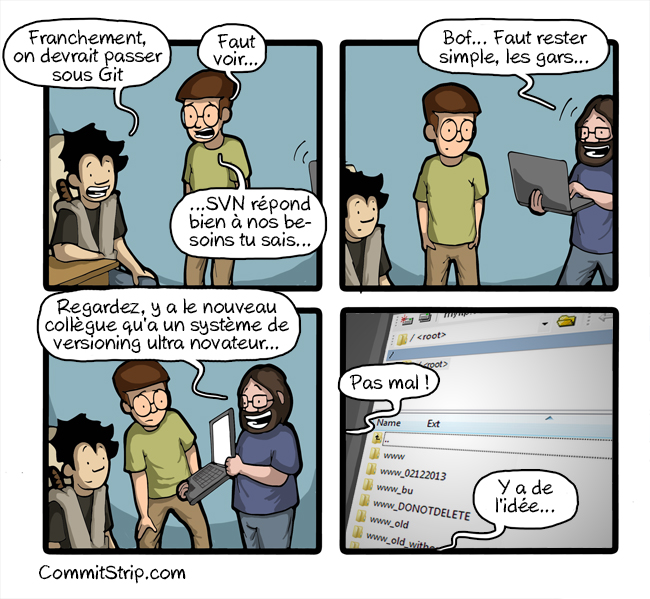
\includegraphics[height=0.8\textheight]{figures/Strips-_Old-650-final1.jpg}
\end{center}

\end{frame}

%%%%%%%%%%%%%%%%%%%%%%%%%%%%%%%%%%%%%%%%%%%%%%%%
% Diapo Git
%%%%%%%%%%%%%%%%%%%%%%%%%%%%%%%%%%%%%%%%%%%%%%%%
\begin{frame}
\frametitle{\texttt{git}}
\framesubtitle{Logiciel de gestion de versions décentralisé}

\begin{itemize}[<+->]
	\item	 Logiciel libre créé par Linus Torvald en 2005
	\item  Permet des sauvegardes successives mais aussi le travail en parallèle de plusieurs personnes sur un même jeu de fichier (penser aux multiples versions des programmes de simulation en TIPE)
	\item  Accessible par la ligne de commande

	(pratique pour scripter mais pas trop pour les élèves)
	\item  Fonctionne en terme de \ofg{commit} qui rassemble des changements atomiques
	\item 	Permet de multiples actions et un suivi historique des modifications successives.

\end{itemize}

\end{frame}


%%%%%%%%%%%%%%%%%%%%%%%%%%%%%%%%%%%%%%%%%%%%%%%%
% Diapo Github
%%%%%%%%%%%%%%%%%%%%%%%%%%%%%%%%%%%%%%%%%%%%%%%%
\begin{frame}
\frametitle{GitHub}
\framesubtitle{Une interface web pour \texttt{git}}

\begin{itemize}[<+->]
	\item Site web permettant un accès centralisé aux repository git (\url{https://github.com})



	\item Sorte de «facebook» des développeurs

	\item Modèle commercial: repositories publics illimités mais privés payant au-delà de 3 collaborateurs (sauf organisations à visées pédagogiques)

\end{itemize}

\end{frame}


%%%%%%%%%%%%%%%%%%%%%%%%%%%%%%%%%%%%%%%%%%%%%%%%
% Diapo Github
%%%%%%%%%%%%%%%%%%%%%%%%%%%%%%%%%%%%%%%%%%%%%%%%
\begin{frame}
\frametitle{GitHub}
\framesubtitle{Exemple du noyau Linux}

	\begin{center}
			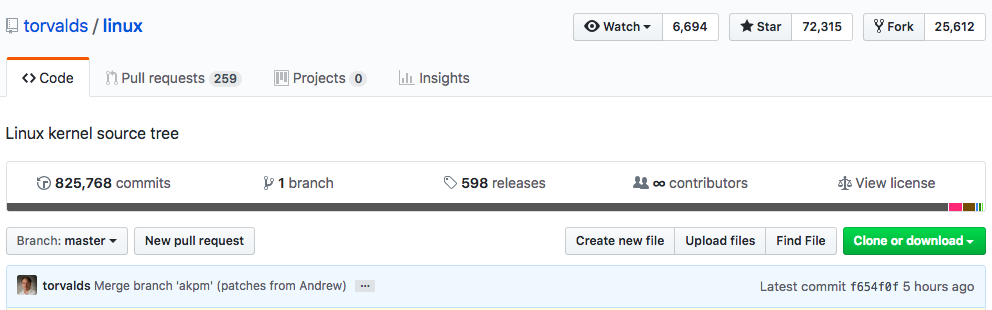
\includegraphics[width=\linewidth]{figures/github_linux.png}
	\end{center}

\end{frame}

%%%%%%%%%%%%%%%%%%%%%%%%%%%%%%%%%%%%%%%%%%%%%%%%
% Diapo Github
%%%%%%%%%%%%%%%%%%%%%%%%%%%%%%%%%%%%%%%%%%%%%%%%
\begin{frame}
\frametitle{GitHub}
\framesubtitle{Exemple de visualisation de compte}

	\begin{center}
			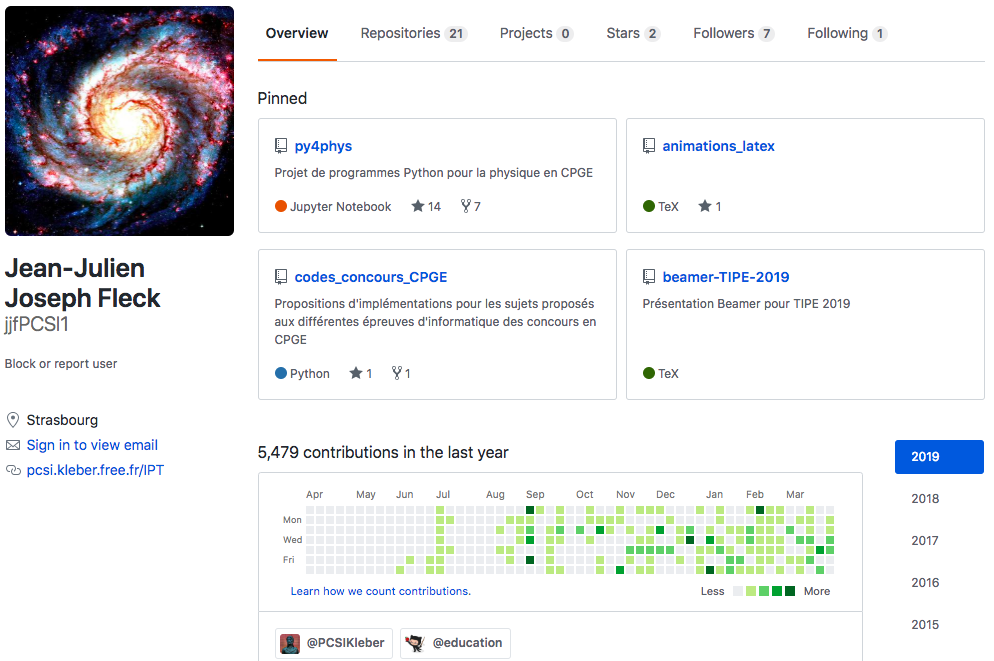
\includegraphics[width=\linewidth]{figures/github_jjfPCSI1.png}
	\end{center}

\end{frame}

%%%%%%%%%%%%%%%%%%%%%%%%%%%%%%%%%%%%%%%%%%%%%%%%
% Diapo github Desktop
%%%%%%%%%%%%%%%%%%%%%%%%%%%%%%%%%%%%%%%%%%%%%%%%
\begin{frame}
	\frametitle{GitHub Desktop}
	\framesubtitle{Interface graphique pour interagir avec GitHub}

	\begin{itemize}[<+->]
		\item Installation facile depuis \url{https://desktop.github.com/}

		\item Permet de rappatrier les repositories depuis GitHub.com sur l'ordinateur en local

		\item Permet de faire les commits depuis l'ordinateur local.

		\item Aucune connexion requise pour les commits (on peut bosser dans le train par exemple), il suffit de penser à «pousser» les modifications une fois la connexion rétablie.

		\item Très loin d'utiliser toutes la puissance de \texttt{git} mais justement utile pour ne pas effrayer les élèves

	\end{itemize}

\end{frame}

%%%%%%%%%%%%%%%%%%%%%%%%%%%%%%%%%%%%%%%%%%%%%%%%
% Diapo github Desktop
%%%%%%%%%%%%%%%%%%%%%%%%%%%%%%%%%%%%%%%%%%%%%%%%
\begin{frame}
	\frametitle{GitHub Desktop}
	\framesubtitle{Exemple de visualisation d'historique}

	\begin{center}
		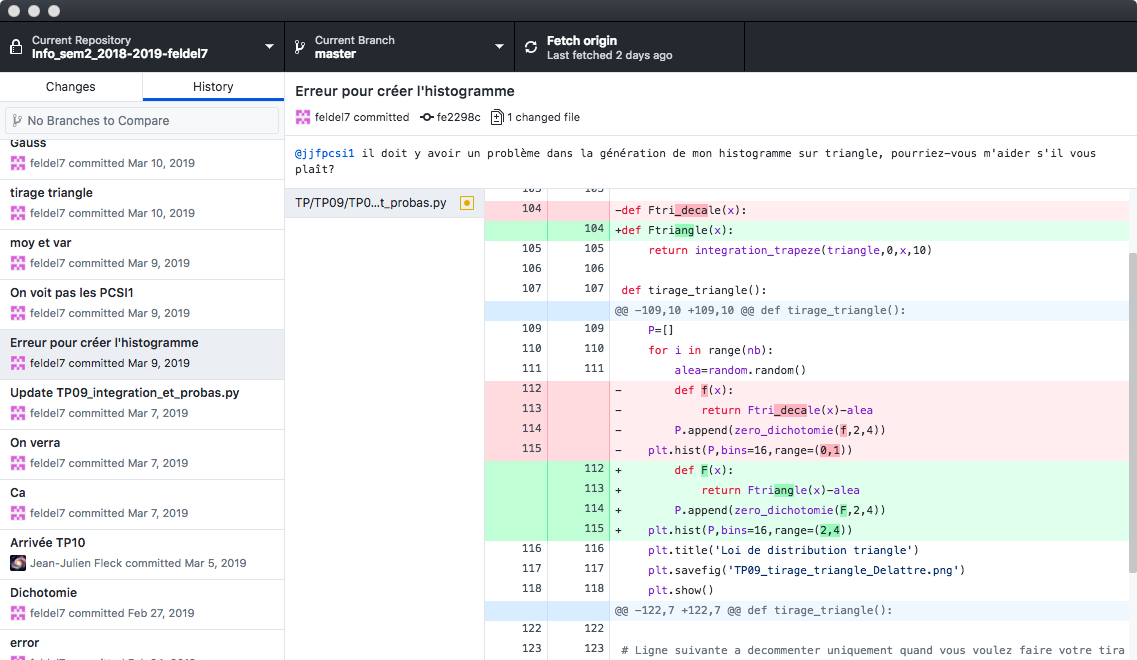
\includegraphics[width=\linewidth]{figures/githubdesktop.png}
	\end{center}

\end{frame}

%%%%%%%%%%%%%%%%%%%%%%%%%%%%%%%%%%%%%%%%%%%%%%%%
% Diapo github Desktop
%%%%%%%%%%%%%%%%%%%%%%%%%%%%%%%%%%%%%%%%%%%%%%%%
\begin{frame}
	\frametitle{GitHub Desktop}
	\framesubtitle{Exemple de visualisation de commit}

	\begin{center}
		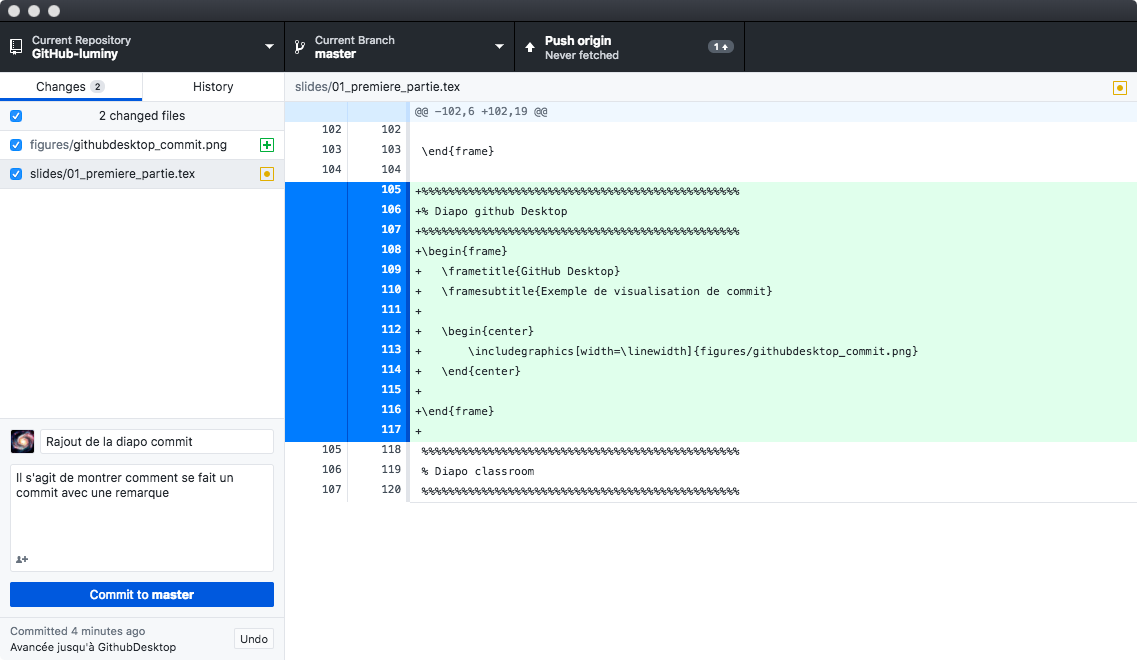
\includegraphics[width=\linewidth]{figures/githubdesktop_commit.png}
	\end{center}

\end{frame}

%%%%%%%%%%%%%%%%%%%%%%%%%%%%%%%%%%%%%%%%%%%%%%%%
% Diapo classroom
%%%%%%%%%%%%%%%%%%%%%%%%%%%%%%%%%%%%%%%%%%%%%%%%
\begin{frame}
	\frametitle{GitHub Classroom \url{https://classroom.github.com/}}
	\framesubtitle{Un service annexe de GitHub}

	\begin{center}
		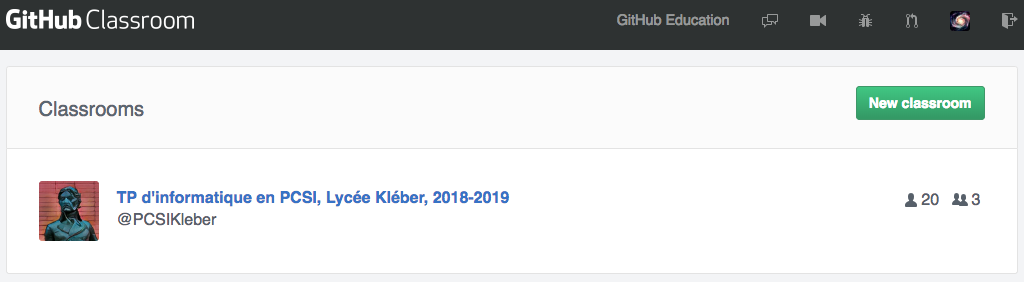
\includegraphics[width=\linewidth]{figures/classroom_accueil.png}
	\end{center}

	\begin{itemize}[<+->]
		\item Automatise le processus de création de repositories pour les élèves

		\item Permet de rappatrier les repositories sur l'ordi prof via «classroom assistant» (\url{https://classroom.github.com/assistant})

	\end{itemize}



\end{frame}


% Exemples d'utilisation et divers avantages
% Titre de la premiere partie
\section{Gestion des TP, nouveau protocole}

%%%%%%%%%%%%%%%%%%%%%%%%%%%%%%%%%%%%%%%%%%%%%%%%
%%%%%%%%%%%%%%%%%%%%%%%%%%%%%%%%%%%%%%%%%%%%%%%%
\begin{frame}
	\frametitle{Gestion des TP}
	\framesubtitle{Organisation après GitHub}

	\begin{itemize}[<+->]
		\item	 Dossier de chaque TP distribué via GitHub depuis n'importe où (souvent la maison), le tout pouvant être préparé à l'avance facilement.

		\item  Travail des élèves sur les ordis du lycée ou leur propre ordi en ayant toujours la dernière version à jour (à condition d'avoir pensé à «pousser» leurs derniers commits)

		\item Ramassage des dossiers des élèves de n'importe où (et à n'importe quelle heure) avec possibilité d'imposer une deadline indépendante de l'aspect matériel (on prend le dernier commit avant la deadline, sans compter les suivants).

		\resizebox{\linewidth}{!}{\texttt{git checkout `git rev-list -n 1 --before="2018-09-15 13:37" master`}}

	\end{itemize}

\end{frame}


%%%%%%%%%%%%%%%%%%%%%%%%%%%%%%%%%%%%%%%%%%%%%%%%
%%%%%%%%%%%%%%%%%%%%%%%%%%%%%%%%%%%%%%%%%%%%%%%%
\begin{frame}
	\frametitle{Gestion des TP}
	\framesubtitle{Avantages élèves}

	\begin{itemize}[<+->]
		\item Sauvegarde et archivage automatique du travail des élèves.

		\item Possibilité de poser des questions lors des commits.

		\visible<2-> {
		\begin{center}
				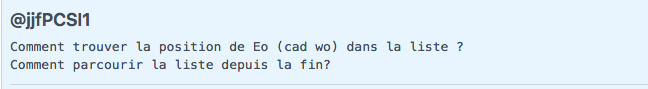
\includegraphics[width=0.8\linewidth]{figures/github_questions_commit.png}
		\end{center}
		}

		\item Feedback possible depuis n'importe où directement dans le code des commits des élèves.

		\visible<3-> {
			\begin{center}
					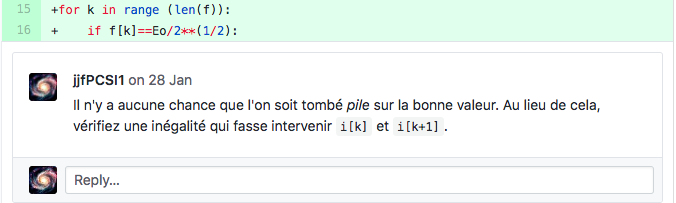
\includegraphics[width=0.8\linewidth]{figures/github_commentaires_commit.png}
			\end{center}
		}

	\end{itemize}

\end{frame}

%%%%%%%%%%%%%%%%%%%%%%%%%%%%%%%%%%%%%%%%%%%%%%%%
%%%%%%%%%%%%%%%%%%%%%%%%%%%%%%%%%%%%%%%%%%%%%%%%
\begin{frame}
	\frametitle{Gestion des TP}
	\framesubtitle{Avantages élèves}

	\begin{center}
		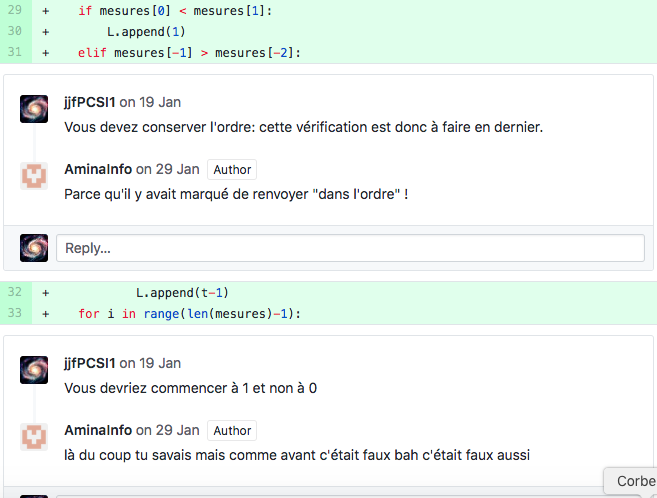
\includegraphics[width=0.8\linewidth]{figures/TP_note_info.png}
	\end{center}

\end{frame}

%%%%%%%%%%%%%%%%%%%%%%%%%%%%%%%%%%%%%%%%%%%%%%%%
%%%%%%%%%%%%%%%%%%%%%%%%%%%%%%%%%%%%%%%%%%%%%%%%
\begin{frame}
	\frametitle{Gestion des TP}
	\framesubtitle{Avantages profs}

	\begin{itemize}[<+->]
		\item Suivi facilité du travail des élèves durant les TP (et au-dehors)

		\item Conseils localisés et personnalisés

		\item Accès direct au code pour identifier les problèmes

		\item Détermination facilitée des fraudeurs potentiels

		\item Gestion entière scriptée, moins de manipulations «manuelles» nécessaires

	\end{itemize}

\end{frame}


% Mise en place pratique
% Titre de la partie
\section{Mise en place de GitHub Classroom}


%%%%%%%%%%%%%%%%%%%%%%%%%%%%%%%%%%%%%%%%%%%%%%%%
%%%%%%%%%%%%%%%%%%%%%%%%%%%%%%%%%%%%%%%%%%%%%%%%
\begin{frame}
	\frametitle{Ensemble du processus}
	%\framesubtitle{}

	Il est décrit dans cette petite vidéo

	\begin{center}
		\url{https://www.youtube.com/watch?v=ChA_zph7aao}
	\end{center}


\end{frame}



%%%%%%%%%%%%%%%%%%%%%%%%%%%%%%%%%%%%%%%%%%%%%%%%
%%%%%%%%%%%%%%%%%%%%%%%%%%%%%%%%%%%%%%%%%%%%%%%%
\begin{frame}
	\frametitle{Création de l'organisation}
	%\framesubtitle{}

	\begin{center}
		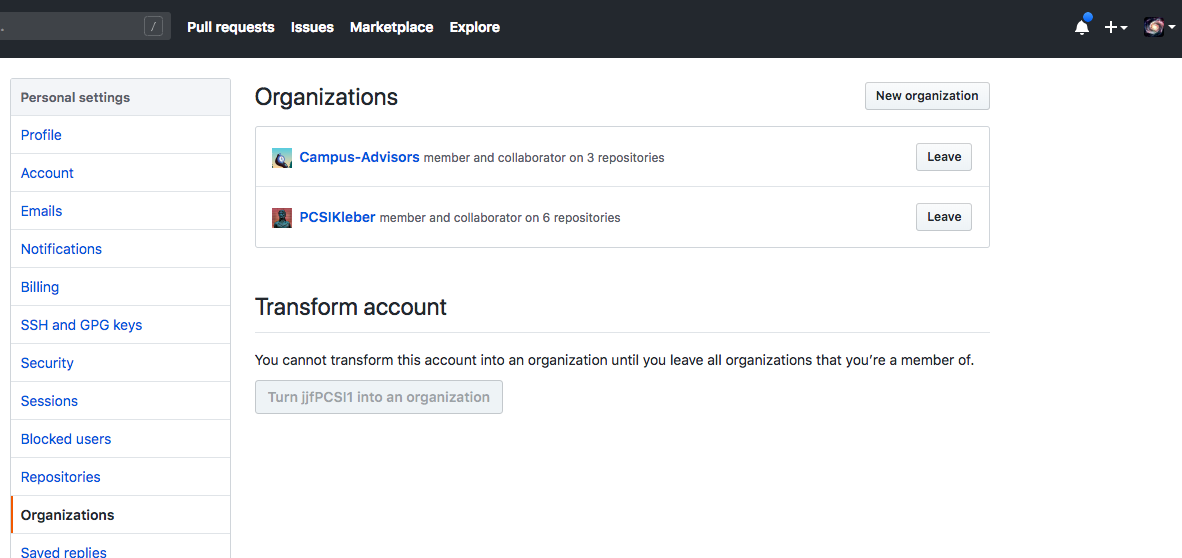
\includegraphics[width=0.8\linewidth]{figures/classroom_organization.png}
	\end{center}

	\begin{itemize}[<+->]
		\item	Depuis \url{github.com}, aller dans «Settings» (en haut à droite sur l'avatar de votre compte)

		\item Puis «Organizations» (onglet en bas à gauche)

		\item Puis «New organisation» (bouton)

	\end{itemize}

\end{frame}


%%%%%%%%%%%%%%%%%%%%%%%%%%%%%%%%%%%%%%%%%%%%%%%%
%%%%%%%%%%%%%%%%%%%%%%%%%%%%%%%%%%%%%%%%%%%%%%%%
\begin{frame}
	\frametitle{Création de la \ofg{classroom}}
	\framesubtitle{Première étape}

	Depuis \url{https://classroom.github.com/classrooms} (après s'être connecté, bien entendu), cliquer sur le bouton «New classroom» (en haut à droite)

	\begin{center}
		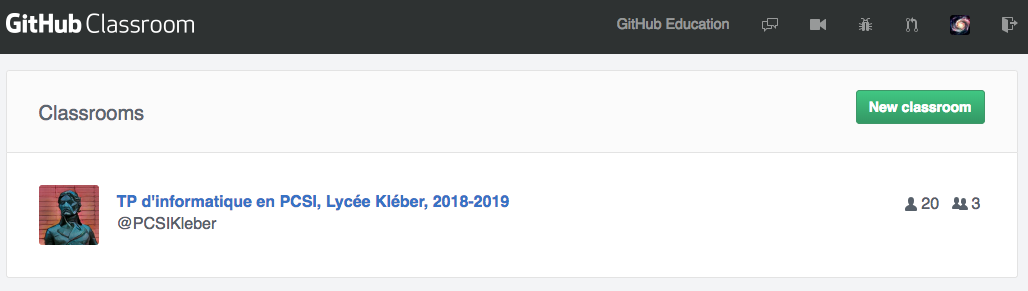
\includegraphics[width=\linewidth]{figures/classroom_new_classroom.png}
	\end{center}

\end{frame}

%%%%%%%%%%%%%%%%%%%%%%%%%%%%%%%%%%%%%%%%%%%%%%%%
%%%%%%%%%%%%%%%%%%%%%%%%%%%%%%%%%%%%%%%%%%%%%%%%
\begin{frame}
	\frametitle{Création de la \ofg{classroom}}
	\framesubtitle{Sélection de l'organization}

	Sélectionner l'«organization» adéquate

	\begin{center}
		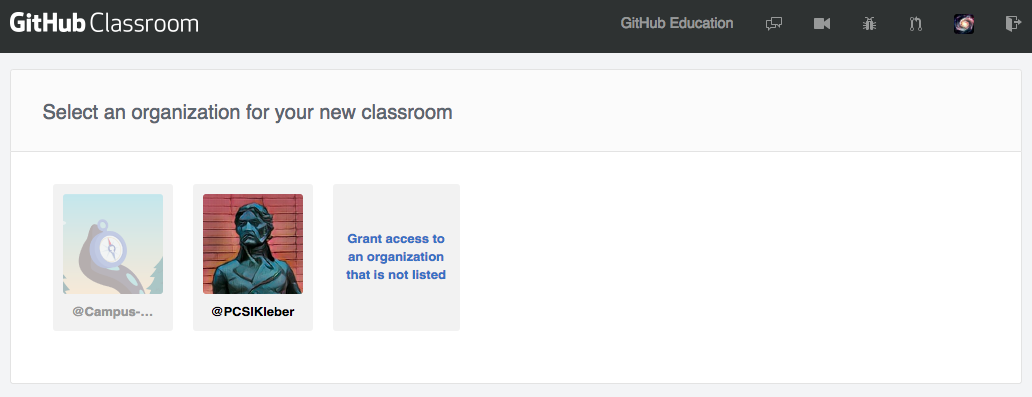
\includegraphics[width=\linewidth]{figures/classroom_select_organization.png}
	\end{center}

\end{frame}

%%%%%%%%%%%%%%%%%%%%%%%%%%%%%%%%%%%%%%%%%%%%%%%%
%%%%%%%%%%%%%%%%%%%%%%%%%%%%%%%%%%%%%%%%%%%%%%%%
\begin{frame}
	\frametitle{Création de la \ofg{classroom}}
	\framesubtitle{Nomination}

	Donner un nom explicite à la classroom

	\begin{center}
		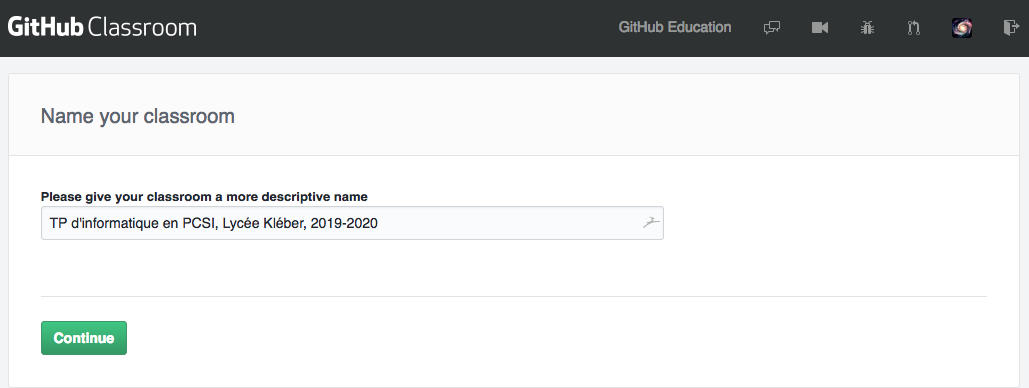
\includegraphics[width=\linewidth]{figures/classroom_naming.png}
	\end{center}

\end{frame}

%%%%%%%%%%%%%%%%%%%%%%%%%%%%%%%%%%%%%%%%%%%%%%%%
% Deuxième diapo
%%%%%%%%%%%%%%%%%%%%%%%%%%%%%%%%%%%%%%%%%%%%%%%%
\begin{frame}
	\frametitle{Création de la \ofg{classroom}}
	\framesubtitle{Invitation d'autres administrateurs}

	%Inscrivez vos collègues à votre organization et donnez-leur le lien vers la classroom

	\begin{center}
		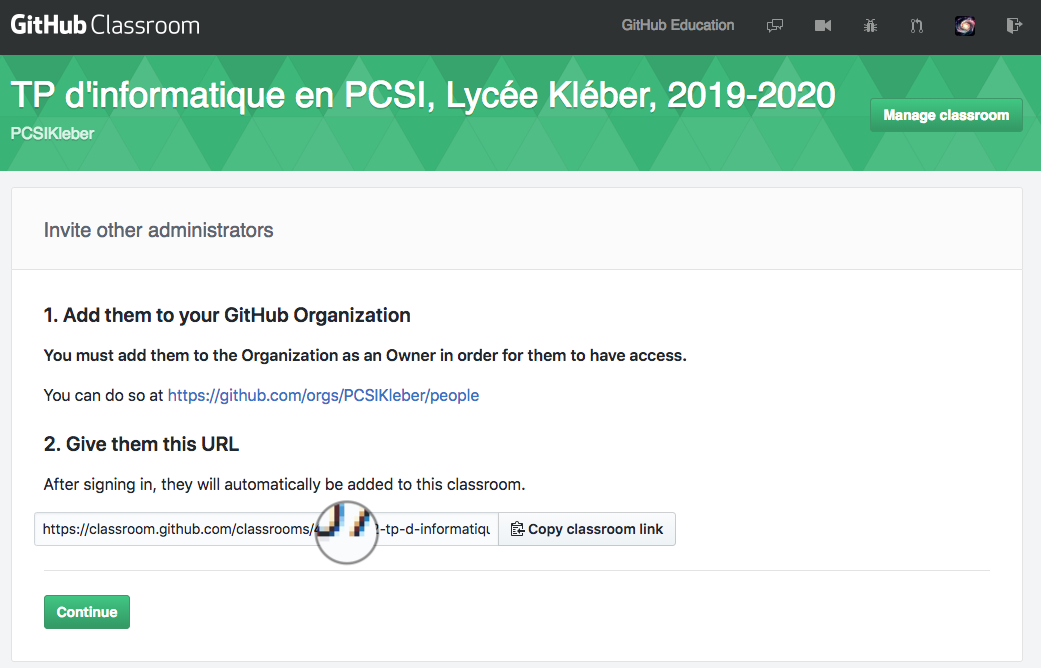
\includegraphics[width=\linewidth]{figures/classroom_invite_admin.png}
	\end{center}

\end{frame}

%%%%%%%%%%%%%%%%%%%%%%%%%%%%%%%%%%%%%%%%%%%%%%%%
% Deuxième diapo
%%%%%%%%%%%%%%%%%%%%%%%%%%%%%%%%%%%%%%%%%%%%%%%%
\begin{frame}
	\frametitle{Création de la \ofg{classroom}}
	\framesubtitle{Préparation du roster}

	%Inscrivez vos collègues à votre organization et donnez-leur le lien vers la classroom

	\begin{center}
		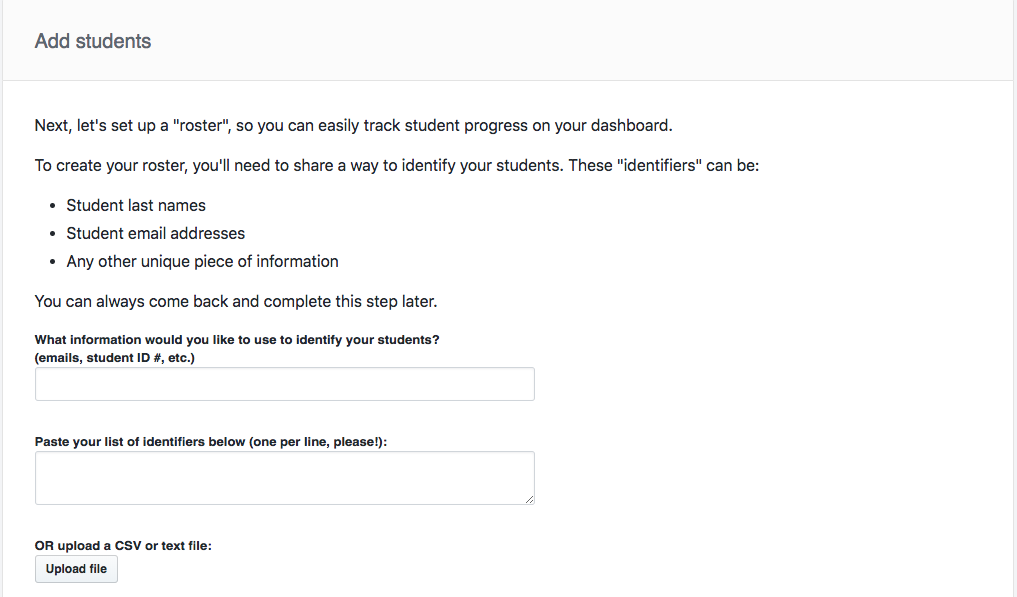
\includegraphics[width=\linewidth]{figures/classroom_roster.png}
	\end{center}

\end{frame}

%%%%%%%%%%%%%%%%%%%%%%%%%%%%%%%%%%%%%%%%%%%%%%%%
%%%%%%%%%%%%%%%%%%%%%%%%%%%%%%%%%%%%%%%%%%%%%%%%
\begin{frame}
	\frametitle{Premier «Assignment»}
	\framesubtitle{Création}

	%Inscrivez vos collègues à votre organization et donnez-leur le lien vers la classroom

	\begin{center}
		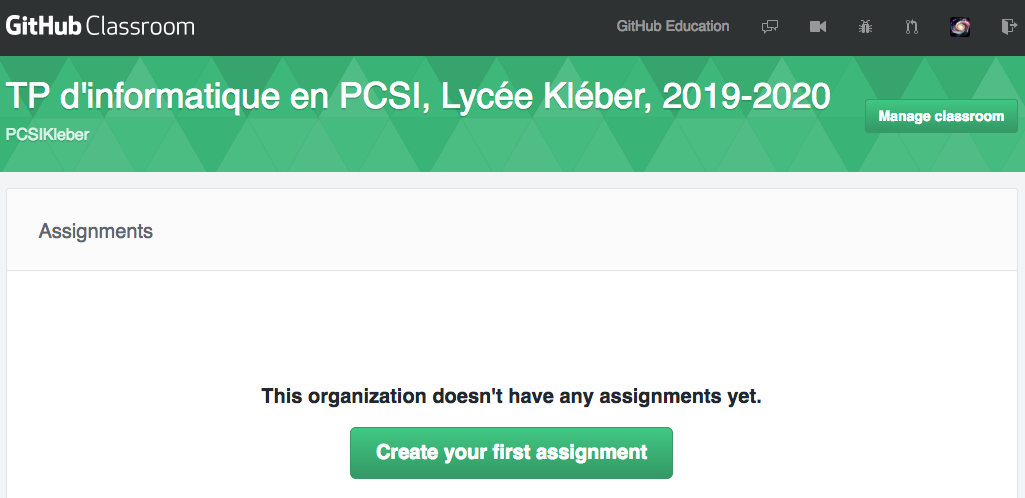
\includegraphics[width=\linewidth]{figures/classroom_assignment_creation.png}
	\end{center}

\end{frame}

%%%%%%%%%%%%%%%%%%%%%%%%%%%%%%%%%%%%%%%%%%%%%%%%
%%%%%%%%%%%%%%%%%%%%%%%%%%%%%%%%%%%%%%%%%%%%%%%%
\begin{frame}
	\frametitle{Premier «Assignment»}
	\framesubtitle{Type}

	%Inscrivez vos collègues à votre organization et donnez-leur le lien vers la classroom

	\begin{center}
		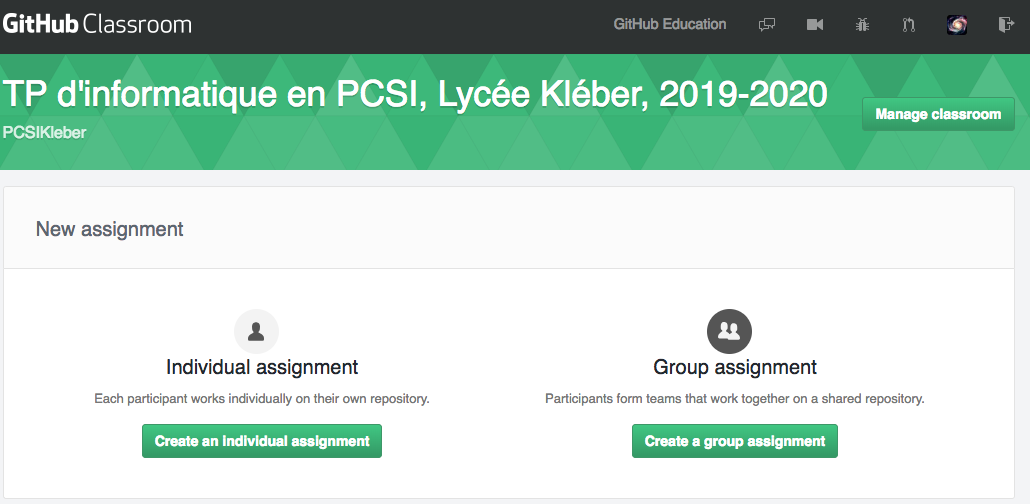
\includegraphics[width=\linewidth]{figures/classroom_assignment_type.png}
	\end{center}

\end{frame}

%%%%%%%%%%%%%%%%%%%%%%%%%%%%%%%%%%%%%%%%%%%%%%%%
%%%%%%%%%%%%%%%%%%%%%%%%%%%%%%%%%%%%%%%%%%%%%%%%
\begin{frame}
	\frametitle{Premier «Assignment»}
	\framesubtitle{Réglages}

	\begin{center}
		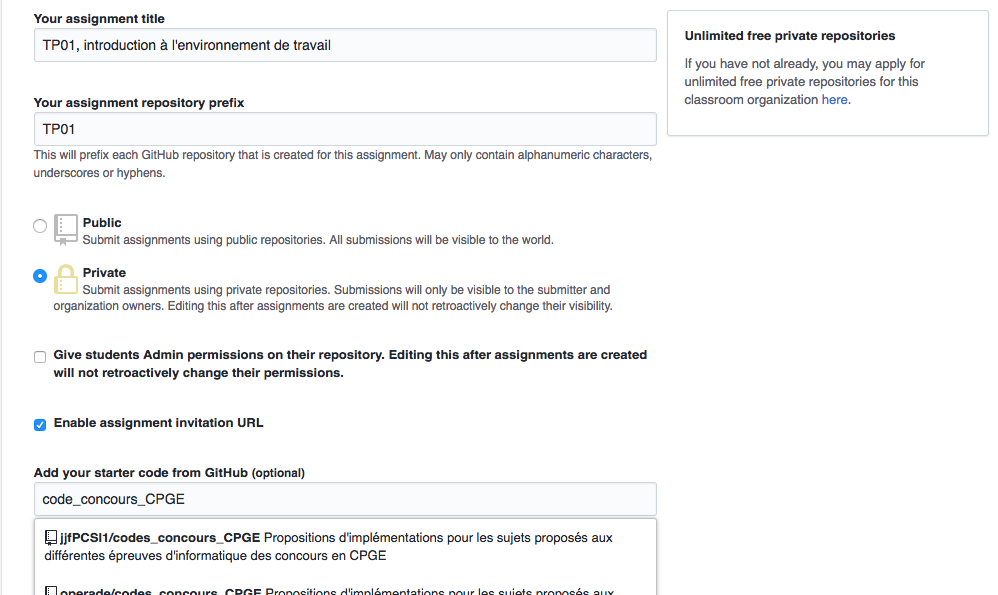
\includegraphics[height=0.8\textheight]{figures/classroom_assignment_reglages.png}
	\end{center}

\end{frame}

%%%%%%%%%%%%%%%%%%%%%%%%%%%%%%%%%%%%%%%%%%%%%%%%
%%%%%%%%%%%%%%%%%%%%%%%%%%%%%%%%%%%%%%%%%%%%%%%%
\begin{frame}
	\frametitle{Premier «Assignment»}
	\framesubtitle{Récupération des dossiers}

	\begin{center}
		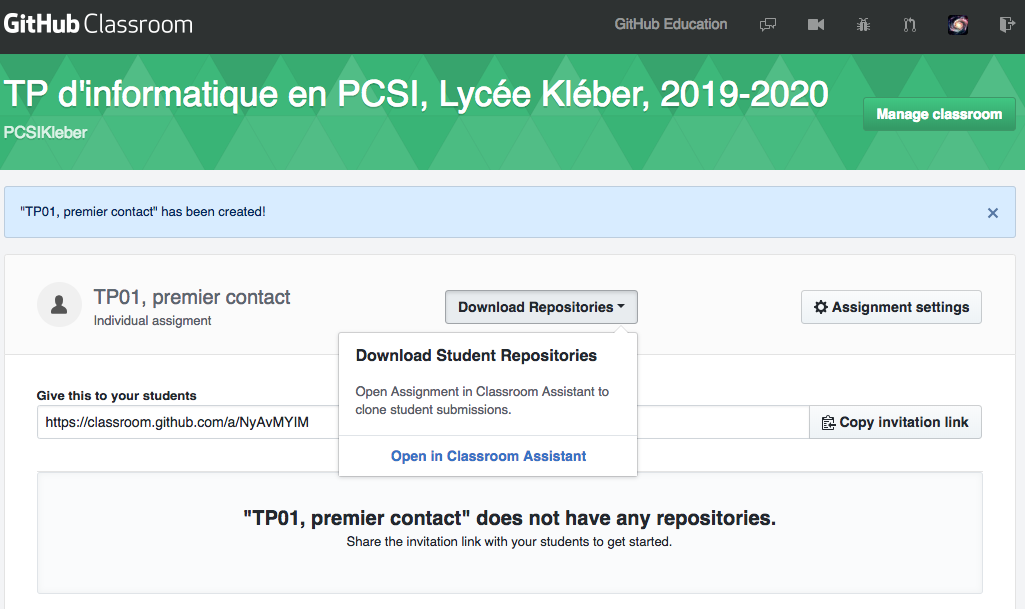
\includegraphics[width=\linewidth]{figures/classroom_assignment_suivi.png}
	\end{center}

\end{frame}


% Structuration des devoirs
% Le titre de la partie
\section{Diverses utilisation possibles}

%%%%%%%%%%%%%%%%%%%%%%%%%%%%%%%%%%%%%%%%%%%%%%%%
% Première diapo
%%%%%%%%%%%%%%%%%%%%%%%%%%%%%%%%%%%%%%%%%%%%%%%%

\begin{frame}
\frametitle{Un devoir par TP par élève}
%\framesubtitle{}

\begin{itemize}
	\item	<1->
\end{itemize}

\end{frame}

%%%%%%%%%%%%%%%%%%%%%%%%%%%%%%%%%%%%%%%%%%%%%%%%
% Deuxième diapo
%%%%%%%%%%%%%%%%%%%%%%%%%%%%%%%%%%%%%%%%%%%%%%%%

\begin{frame}
\frametitle{Un dossier semestriel par élève}
%\framesubtitle{}

\begin{itemize}
	\item	<1->
\end{itemize}

\end{frame}

%%%%%%%%%%%%%%%%%%%%%%%%%%%%%%%%%%%%%%%%%%%%%%%%
% Diapo exemple: le code informatique impose un
% environnement "fragile" pour la frame
%%%%%%%%%%%%%%%%%%%%%%%%%%%%%%%%%%%%%%%%%%%%%%%%

\begin{frame}[fragile]
\frametitle{Relativité Générale}
\framesubtitle{Le code informatique}

\begin{code}
\begin{minted}[linenos]{python}

import scipy as sp
import scipy.optimize

def ma_fonction(x):
    return []

# À vous de remplir les choses adéquates...

\end{minted}
\end{code}
\end{frame}


% Conclusion
% Le titre de la partie
\section{Conclusions}

%%%%%%%%%%%%%%%%%%%%%%%%%%%%%%%%%%%%%%%%%%%%%%%%
%%%%%%%%%%%%%%%%%%%%%%%%%%%%%%%%%%%%%%%%%%%%%%%%
\begin{frame}
  \frametitle{Conclusions}
  

  \begin{itemize}[<+->]
      \item Une expérience très positive

      \item Accueil favorable des élèves: pas plus compliqué de leur point de vue que prendre un IDE en main (mais pour les collègues, c'est une autre histoire)

      \item Permet un suivi bien meilleur des élèves

      \item Structure choisie pour l'année prochaine:
        \begin{itemize}
            \item Un unique repository pour l'année avec rajouts réguliers de nouveaux répertoires

            \item Cahier de TP de physique introduit tout de suite et partagé sur la classe
        \end{itemize}

  \end{itemize}

\end{frame}


\end{document}
